\documentclass[../../../interview-questions.tex]{subfiles}

\begin{document}

\subsection{\color{red}{Java NIO原理}}

NIO(在Java领域,也称为New I/O),注意Non-blocking I/O与New I/O是不一样的\footnote{具体可参考:\url{https://www.51cto.com/article/630142.html}},Java NIO(New IO) 不是IO模型中的NIO模型,而是另外的一种模型,叫做IO多路复用模型( IO multiplexing ),是一种同步非阻塞的I/O模型,也是I/O多路复用的基础,已经被越来越多地应用到大型应用服务器,成为解决高并发与大量连接、I/O处理问题的有效方式。NIO由原来的阻塞读写(占用线程)变成了单线程轮询事件,找到可以进行读写的网络描述符进行读写。除了事件的轮询是阻塞的(没有可干的事情必须要阻塞),剩余的I/O操作都是纯CPU操作,没有必要开启多线程。并且由于线程的节约,连接数大的时候因为线程切换带来的问题也随之解决,进而为处理海量连接提供了可能。单线程处理I/O的效率确实非常高,没有线程切换,只是拼命的读、写、选择事件。但现在的服务器,一般都是多核处理器,如果能够利用多核心进行I/O,无疑对效率会有更大的提高。
Netty 实际上就基于 Java NIO 技术封装完善之后得到一个高性能框架,熟悉 NIO 的基本概念对于学习和更好地理解 Netty 还是很有必要的!NIO由一个专门的线程处理所有IO事件,并负责分发。事件驱动机制,事件到来的时候触发操作,不需要阻塞的监视事件。线程之前通过wait,notify通信,减少线程切换。

\begin{figure}[htbp]
	\centering
	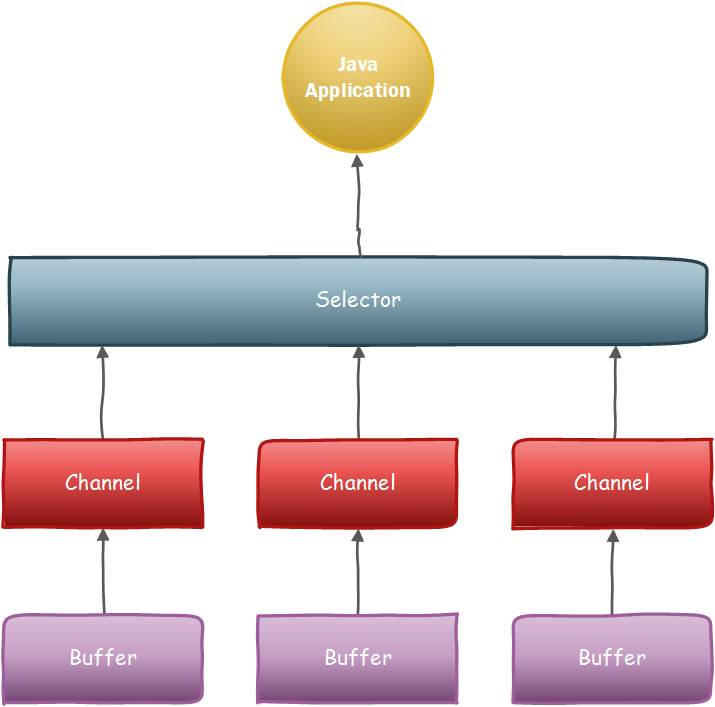
\includegraphics[scale=0.3]{nio-selector.png}
	\caption{NIO模型}
	\label{fig:nioselector}
\end{figure}


NIO主要有三大核心部分:Channel(通道),Buffer(缓冲区), Selector(选择器)。传统IO基于字节流和字符流进行操作,而NIO基于Channel和Buffer(缓冲区)进行操作,数据总是从通道读取到缓冲区中,或者从缓冲区写入到通道中。Selector(选择区)用于监听多个通道的事件(比如:连接打开,数据到达)。因此,单个线程可以监听多个数据通道。

\textbf{Channel} Channel是所有访问IO设备的统称。类型与IO中的Stream,而通道是双向的,既可以读又可以写,但是Stream是单项的。常用的通道有:SocketChannel和ServerSocketChannel(对应TCP的客户端和服务器端)、FileChannel(对应文件IO)、DatagramChannel(对应UDP)等

\textbf{Buffer}所有数据的读写都要经过Buffer,Buffer直接和Channel打交道,是一个存储数据的容器。通过调用Channel.write方法将数据写入Buffer,Channel.read方法将数据从Buffer中读取出来。常用的Buffer有:ByteBuffer、LongBuffer、IntBuffer、StringCharBuffer等

\textbf{Selector}Selector用来监听多个Channel的事件(比如:Read、Write、Connect和Accept等),通过单个线程轮询的方式实现了对多个Channel的监听。Java NIO根据操作系统不同, 针对NIO中的Selector有不同的实现。



\paragraph{NIO与epoll}

Java NIO根据操作系统不同, 针对NIO中的Selector有不同的实现:

\begin{enumerate}
\item{macosx:KQueueSelectorProvider}
\item{solaris:DevPollSelectorProvider}
\item{Linux:EPollSelectorProvider (Linux kernels >= 2.6)或PollSelectorProvider}
\item{windows:WindowsSelectorProvider}
\end{enumerate}
所以不需要特别指定,Oracle JDK会自动选择合适的Selector。如果想设置特定的Selector,可以设置属性,例如:
\url{-Djava.nio.channels.spi.SelectorProvider=sun.nio.ch.EPollSelectorProvider}

JDK在Linux已经默认使用epoll方式,但是JDK的epoll采用的是水平触发(level-triggered),在水平触发的情况下,必须不断的轮询监控每个文件描述符的状态,判断其是否可读或可写。内核空间中维护的 I/O 状态列表可能随时会被更新,因此用户程序想要拿到 I/O 状态列表必须访问内核空间。所以Netty自4.0.16起, Netty为Linux通过JNI的方式提供了native socket transport。Netty重新实现了epoll机制,采用边缘触发(edge-triggered)方式,而边缘触发的情况下,只有在数据到达网卡,也就是说 I/O 状态发生改变时才会触发事件,在两次数据到达的间隙,I/O 状态列表是不会发生改变的。这就使得用户程序可以缓存一份 I/O 状态列表在用户空间中,减少系统调用的次数。
netty epoll transport暴露了更多的nio没有的配置参数,如 TCP\_CORK, SO\_REUSEADDR等等。
C代码,更少GC,更少synchronized
使用native socket transport的方法很简单,只需将相应的类替换即可。


\paragraph{Java IO与NIO的区别}

NIO是一种叫非阻塞IO(Non-blocking I/O),基于I/O多路复用来实现的(可参考:I/O模型、select、poll和epoll之间的区别)。NIO与之前传统的I/O模型有很大的不同,具体表现在以下几个方面:

面向流与面向缓冲
Java IO和NIO之间一个最大的区别是,IO是面向流的,NIO是面向缓冲区的。Java IO每次从数据流中读一个或多个字节,直至读取所有字节,数据流是一次性的,读取完以后,不能前后移动流中的数据。Java NIO是将数据读取到缓冲区,可以通过position来回移动访问缓冲区中的数据。

阻塞与非阻塞IO
Java IO中调用read和write方法的线程会被阻塞的,直到数据全部读入或者全部写入完为止。而在Java NIO中,如果需要读写数据只用和缓冲区打交道,将数据从缓冲区读取或者写入缓冲区以后,线程可以继续做其他事情,不会被block住。

选择器(Selector)
Selector是基于I/O多路复用的机制实现的,将多个Channel注册到一个Selector上,Selector通过轮询监听所有注册的通道上是否有SelectionKey发生,如果发生了,然后将SelectionKey分派给其他线程处理。

\end{document}